\documentclass[10pt,a4paper]{article}
\usepackage[UTF8,fontset = windows]{ctex}
\setCJKmainfont[BoldFont=黑体,ItalicFont=楷体]{华文中宋}
\usepackage{amssymb,amsmath,amsfonts,amsthm,mathrsfs,dsfont,graphicx}
\usepackage{ifthen,indentfirst,enumerate,color,titletoc}
\usepackage{tikz}
\usepackage{makecell}
\usepackage{longtable}

\usetikzlibrary{arrows,calc,intersections,patterns}
\usepackage[bf,small,indentafter,pagestyles]{titlesec}
\usepackage[top=1in, bottom=1in,left=0.8in,right=0.8in]{geometry}
\renewcommand{\baselinestretch}{1.65}
\newtheorem{defi}{定义~}
\newtheorem{eg}{例~}
\newtheorem{ex}{~}
\newtheorem{rem}{注~}
\newtheorem{thm}{定理~}
\newtheorem{coro}{推论~}
\newtheorem{axiom}{公理~}
\newtheorem{prop}{性质~}
\newcommand{\blank}[1]{\underline{\hbox to #1pt{}}}
\newcommand{\bracket}[1]{(\hbox to #1pt{})}
\newcommand{\onech}[4]{\par\begin{tabular}{p{.9\textwidth}}
A.~#1\\
B.~#2\\
C.~#3\\
D.~#4
\end{tabular}}
\newcommand{\twoch}[4]{\par\begin{tabular}{p{.46\textwidth}p{.46\textwidth}}
A.~#1& B.~#2\\
C.~#3& D.~#4
\end{tabular}}
\newcommand{\vartwoch}[4]{\par\begin{tabular}{p{.46\textwidth}p{.46\textwidth}}
(1)~#1& (2)~#2\\
(3)~#3& (4)~#4
\end{tabular}}
\newcommand{\fourch}[4]{\par\begin{tabular}{p{.23\textwidth}p{.23\textwidth}p{.23\textwidth}p{.23\textwidth}}
A.~#1 &B.~#2& C.~#3& D.~#4
\end{tabular}}
\newcommand{\varfourch}[4]{\par\begin{tabular}{p{.23\textwidth}p{.23\textwidth}p{.23\textwidth}p{.23\textwidth}}
(1)~#1 &(2)~#2& (3)~#3& (4)~#4
\end{tabular}}
\begin{document}
\begin{enumerate}[1.]

\item 写出集合$\{1,2\}$的所有子集.
\item 已知集合$A=\{x|1 \le x<3,\ x\in \mathbf{R}\}$, $B=\{x|x>2,\ x\in \mathbf{R}\}$. 求$A\cap B$, $A\cup B$.
\item 已知集合$U =\{x|x\text{取不大于}30\text{的质数}\}$, $A$, $B$是$U$的两个子集, 且满足$A\cap \complement_UB=\{5,13,23\}$, $\complement_A\cap B=\{11,19,29\}$, $\complement_UA\cap \complement_UB=\{3,7\}$, 求$A$, $B$.
\item 已知集合$A=\{x|x^2- ax+a^2-19=0\}$, $B=\{x|x^2-5x+6=0\}$, $C=\{ x|x^2+2x-8=0\}$满足$A\cap B\ne \varnothing$, $A\cap C=\varnothing$, 求实数$a$的值.
\item 已知集合$A=\{x|x^2-5x+4\le 0\}$与$B=\{x|x^2-2ax+a+2\le 0,\ a\in \mathbf{R}\}$满足$B\subseteq A$, 求$a$的取值范围.
\item 已知集合$A=\{x|x^2 +(\rho +2)x+1=0, \ x\in \mathbf{R}\}$, 且$A\cap \mathbf{R}^+=\varnothing$, 求实数$\rho$的取值范围.
\item 在``\textcircled{1} 难解的题目, \textcircled{2} 方程$x^2+1=0$在实数集内的解, \textcircled{3} 直角坐标平面内第四象限的一些点, \textcircled{4} 很多多项式''中, 能够组成集合的是\bracket{20}.
\fourch{\textcircled{2}}{\textcircled{1}\textcircled{3}}{\textcircled{2}\textcircled{4}}{\textcircled{1}\textcircled{2}\textcircled{4}}
\item 集合$M=\{(x,y)|xy\ge 0,\ x\in \mathbf{R},\ y\in \mathbf{R}\}$是指\bracket{20}.
\twoch{第一象限内的点集}{第三象限内的点集}{在第一、三象限内的点集}{不在第二、四象限内的点集}
\item 下列四个关系中, 正确的是\bracket{20}.
\fourch{$\varnothing \in \{a\}$}{$a\notin \{a\}$}{$\{a\}\in \{a,b\}$}{$a\in \{a,b\}$}
\item 方程组$\begin{cases} 2x+y=0, \\ x-y+3=0 \end{cases}$的解集是\bracket{20}.
\fourch{$\{-1,2\}$}{$(-1,2)$}{$\{(-1,2)\}$}{$\{(x,y)|x=-1, \ y=2\}$}
\item 下列各题中的$M$与$P$表示同一个集合的是\bracket{20}.
\onech{$M=\{(1,-3)\}$, $P=\{(-3,1)\}$}{$M=\varnothing$, $P=\{0\}$}{$M=\{y|y=x^2+1, \ x\in \mathbf{R}\}$, $P=\{(x,y)|y=x^2+1, \ x\in \mathbf{R}\}$}{$M=\{y|y=x^2+1,\ x\in \mathbf{R}\},P\{t|t=(y-1)^2+1, \ y\in \mathbf{R}\}$}
\item 用列举法表示下列各集合.\\
(1) 不大于$6$的非负数整数所组成的集合:\blank{50};\\
(2) 方程$x^3-x^2-x+1=0$的解所组成的集合:\blank{50};\\
(3) $\{y|y=x^2-1, \ |x|\le 2, \ x\in \mathbf{Z}\}$:\blank{50};\\
(4) $\{(x,y)|y =x^2-1, \  |x|\le 2,\ x\in \mathbf{Z}\}$:\blank{50};\\
(5) $\{(x,y)|x+y=5, \ x\in \mathbf{N},\ y\in \mathbf{Z}\}$:\blank{50}.
\item 若集合$M=\{0,2,3,7\},P=\{x|x=ab, \ a,b\in M, \ a\ne b\}$, 则$a=$\blank{50}(用列举法表示).
\item 若集合$M=\{x|ax^2+2x+1=0\}$只含一个元素, 则$a=$\blank{50}.
\item 已知集合$A=\{\text{小于}6\text{的自然数}\}$, $B=\{\text{小于}10\text{的质数}\}$, $C=\{24\text{和}36\text{的正公约数}\}$, 用列举法表示:\\
(1) $\{y|y\in A\text{且}y\in C\}$;\\
(2) $\{y|y\in B\text{且}y\notin C\}$.
\item 已知集合$A=\{x|\dfrac{12}{5-x}\in \mathbf{N},\ x\in\mathbf{Z}\}$, 用列举法表示集合$A$.
\item 已知集合$M=\{a,a+d,a+2d\}$, $N=\{a,aq,aq^2\}$, 其中$a\ne 0$, $M=N$, 求$q$的值.
\item 已知集合$A=\{x|x=m^2-n^2, \ m,n\in \mathbf{Z}\}$, 求证:\\
(1) 任何奇数都是$A$的元素;\\
(2) 偶数$4k-2$($k\in \mathbf{Z}$)不属于$A$.
\item 数0与空集$\varnothing$之间的关系是\bracket{20}
\fourch{$0\in \varnothing$}{$0\notin \varnothing$}{$0=\varnothing$}{$0\subset \varnothing$}14.若集合$M=\{x |x\le 6\},a=\sqrt 5$, 则下面结论正确的是\bracket{20}
\fourch{$\{ a\}\subset M$}{$a\subset M$}{$\{ a\}\notin M$}{$a\notin M$}15.已知集合$M=\{y |y=x^2-2x-1,x\in \mathbf{R}\},P=\{x |-2\le x\le 4,x\in \mathbf{R}\}$, 则$M$与$P$之间的关系是\bracket{20}
\fourch{$M=P$}{$M\subset P$}{$M\supset P$}{$M\not\subset P$且$M\not\supset P$}
\item 设集合$M=\{ (x,y)| x+y>0,xy>0 \}$, $T=\{ (x,y)| x>0,y>0 \}$, 则$M$与$T$的关系是\bracket{20}
\fourch{$M\supset T$}{$M=T$}{$M\subset T$}{$M\not\subset T$且$M\not\supset T$}
\item 用适合的符号($\in,\notin,=,\subset,\supset$)填空:\\
(1) $3.14$\blank{50}$\mathbf{Q}$; (2) $\{3.14\}$\blank{50}$\mathbf{Q}$; (3) $\{x|x=2k+1,\ k\in \mathbf{Z}\}$\blank{50}$\{x|x=2k-1,\ k\in\mathbf{Z}\}$.
\item 若集合$A=\{x|-3<x<5\}$与$B=\{x|x<a\}$满足$A\subset B$, 则实数$a$的取值范围是\blank{50}.
\item 若集合$A=\{x|(x+1)(2-x)<0\}$, $B=\{x|4x+p<0\}$, 且$B\subset A$, 则实数$p$的取值范围是\blank{50}.
\item 若集合$A=\{x|x^2+x-6=0\}$与$B=\{y|ay+1=0\}$满足$B\subset A$, 则实数$a$所能取得一切值为\blank{50}.
\item (1) 满足$\{a,b\}\subseteq A\subset \{a,b,c\}$的集合$A$有\blank{50}个;\\
(2) 满足$\{1,2,3\}\subset B\subseteq \{ 1,2,3,4,5\}$的集合$B$有\blank{50}个.
\item 满足$M\subseteq \{0,1,2\}$且$M\subseteq \{0,2,4\}$的集合M有\bracket{20}.
\fourch{$1$个}{$2$个}{$3$个}{$4$个}
\item 集合$\{1,2,3\}$的子集个数是\bracket{20}.
\fourch{$6$}{$7$}{$8$}{$9$}
\item 数集$X=\{(2n+1)\pi|n\in \mathbf{Z}\}$与数集$Y=\{(4k\pm 1)\pi|k\in \mathbf{Z}\}$之间的关系是\bracket{20}.
\fourch{$X\subset Y$}{$X\supset Y$}{$X=Y$}{$X\ne Y$}
\item 已知非空集合$P$满足: \textcircled{1} $P\subseteq \{1,2,3,4,5\}$; \textcircled{2} 若$a\in P$, 则$6-a\in P$. 符合上述要求的集合P的个数是\bracket{20}.
\fourch{$4$}{$5$}{$7$}{$31$}
\item 设集合$A=\{0,1\}$, 集合$B=\{x|x\subseteq A\}$, 则$A$与$B$的关系是\blank{50}.
\item 已知集合$A=\{x|-2\le x\le 5\}$, $B=\{x|m+1\le x\le 2m-1\}$满足$B\subseteq A$, 求实数$m$的取值范围.
26.已知集合$M=\{x|-3<x<2\}$, $P=\{x|x<-\sqrt 2\text{或}x>\sqrt 2\}$, 那么$M\cap P$是\bracket{20}.
\twoch{$\{x|-3<x<-\sqrt 2\text{或}\sqrt 2<x<2\}$}{$\mathbf{R}$}{$\{x|-3<x<-\sqrt 2\}$}{$\{x|\sqrt 2<x<2\}$}
\item 若集合$P=\{y|y =x^2+1,\ x\in \mathbf{R}\}$, $Q=\{y|y=x+1, \ x\in \mathbf{R}\}$, 则$P\cap Q$是\bracket{20}.
\fourch{$\{(0,1),(1,2)\}$}{$\{0,1\}$}{$\{1,2\}$}{$\{y|y \ge 1\}$}
\item 若集合$M=\{(x,y)|x+y=0\}$, $P=\{(x,y)|x-y=2\}$, 则$M\cap P$是\bracket{20}.
\fourch{$(1,-1)$}{$\{x=1\}\cup \{y=-1\}$}{$\{1,-1\}$}{$\{(1,-1)\}$}
\item 若$P\cap S=\varnothing$, 且$M=\{P\text{的子集}\}$, $N=\{S\text{的子集}\}$, 则下列各式中一定成立的是\bracket{20}.
\fourch{$M\cap N=\varnothing$}{$M\cap N=\{\varnothing\}$}{$M\cap N\subset P\cap S$}{$M\cap N\supset P\cap S$}
\item 已知$P,M$是非空集合, 且$P\ne M$, 则必定有\bracket{20}.
\fourch{$\varnothing \in P\cap M$}{$\varnothing=P\cap M$}{$\varnothing \subseteq P\cap M$}{$\varnothing \subset P\cap M$}
\item 若集合$P$, $S$满足$P\cap S=P$, 则下列关系式中恒成立的是\bracket{20}.
\fourch{$P\subset S$}{$P\subseteq S$}{$P=S$}{$P\supset S$}
\item 已知集合$A=\{\text{平行四边形}\}$, $B=\{\text{梯形}\}$, $C=\{\text{对角线相等的四边形}\}$, 那么$B\cap C$=\blank{50}, $A\cap C=$\blank{50}.
\item 若集合$P=\{y|y=x^2-6x+10\}$, $M=\{y|y=-x^2+2x+8\}$, 则$P\cap M=$\blank{50}.
\item 若集合$S=\{x|x\le 2\text{或}x\ge 3\}$, $T=\{x|2\le x\le 3\}$, 则$S\cap T=$\blank{50}.
\item 已知集合$A=\{x|-2\le x\le 4\}$, $B=\{x|x<a\}$, 且满足$A\cap B\ne \varnothing$, 那么实数$a$的取值范围是\blank{50}.
\item 已知集合$P=\{x|-1<x<3\}$, $M=\{x|a<x<2a\}$($a>0$), 且$P\cap M=\varnothing$, 则实数$a$的取值范围是\blank{50}.
\item 记集合$P=\{\text{等腰三角形}\}$, $T=\{\text{至少有一边为}1, \ \text{至少有一内角为}36^\circ\text{的三角形}\}$, 则$P\cap T$的元素有\bracket{20}.
\fourch{$2$个}{$3$个}{$4$个}{$5$个}
\item 若集合$M=\{(x,y)|x-y=0\}$, $P=\{(x,y)|x+y+2=0\}$, 则$M\cap P$=\blank{50}.
\item 若集合$A=\{(x,y)|x^2=y^2\}$, $B=\{(x,y)|y^2=x\}$, 则$A\cap B=$\blank{50}
\item 若集合$A=\{y|y =x^2\}$, $B=\{y|y=1-\sqrt x, \ x\ge 0\}$, 则$A\cap B=$\blank{50}.
\item (1) 已知集合$A=\{2,3,a^2+1\}$, $B=\{a^2+a-4,2a+1,-\dfrac{13}4\}$, 且$A\cap B=\{2\}$, 求实数$a$的值;\\
(2) 已知集合$P=\{m^2,m+1,-3\}$, $Q=\{m-3,2m-1,m^2+1\}$, 且$P\cap Q=\{-3\}$, 求实数$m$的值.
\item 已知集合$M=\{2,3,m^2+4m+2\}$, $P=\{0,7,m^2+4m-2,2-m\}$, 且$M\cap P=\{3,7\}$, 求实数$m$的值和集合$P$.
\item 已知集合$A=\{2,4,a^3-2a^2-a+7\}$, $B=\{-4,a-3,a^2-2a+2,a^3+a^2+3a+7\}$满足$A\cap B=\{2,5\}$, 求实数$a$的值.
\item 已知集合$P=\{x|x^2-ax+a^2-8a+19=0\}$, $Q=\{x|x^2-4x+3=0\}$, $R=\{x|x^2-7x+12=0\}$, 且$P\cap Q\ne \varnothing$, $P\cap R=\varnothing$, 求实数$a$的值.
\item 已知集合$P=\{x|-2\le x\le 5\}$, $Q=\{x|k+1\le x\le 2k-1\}$, 求使$P\cap Q=\varnothing$的实数$k$的取值范围.
\item 若集合$M=\{y|y=x^2+1, \ x\in \mathbf{R}\}$, $P=\{y|y=5-x^2, \ x\in \mathbf{R}\}$, 则$M\cup P$等于\bracket{20}.
\fourch{$\mathbf{R}$}{$\{y|1\le y\le 5\}$}{$\{x|-5\le x\le 1\}$}{$\{(-\sqrt 2,3),(\sqrt 2,3)\}$}
\item 43.集合$M=\{x |x=t^2+3t+2,\ t\in \mathbf{R}\}$与$P=\{y |y=k^2-3k+2,\ k\in \mathbf{R}\}$之间的关系是\bracket{20}.
\twoch{$M\cap P=\varnothing$}{$M\cap P=\{ 0\}$}{$M\cap P=\{(x,y)|x \in \mathbf{R}, \ y  \in \mathbf{R}\}$}{$M\cap P$}
\item 设集合$M=\{x|a_1x^2+b_1x+c_1=0\}$, $N=\{x|a_2x^2+b_2x+c_2=0\}$, 方程$(a_1x^2+b_1x+c_1)(a_2x^2+b_2x+c_2)=0$的解集是\bracket{20}.
\item 在\textcircled{1} $(M\cap P)\subset P$; \textcircled{2} $(M\cup P)\subset P$; \textcircled{3} $(M\cap P)\subset (M\cup P)$; \textcircled{4} 若$M\subset P$, 则$M\cap P=M$这四个结论中, 正确的个数是 \bracket{20}.
\fourch{$1$}{$2$}{$3$}{$4$}
\item 若集合$M$, $P$满足$M\cap P=P$, 则一定有\bracket{20}.
\fourch{$M=P$}{$M\subset P$}{$M\cup P=M$}{$P\subset M$}
\item 若$M$, $P$是两个非空集合, 且对于$M$中的任何一个元素$x$, 都有$x\notin P$, 则有\bracket{20}.
\fourch{$M\supseteq P$}{$M\subseteq P$}{$M\cap P=\varnothing$}{$M\cup P=M$}
\item 若集合$P=\{x|1<x<4\}$, $Q=\{x|x>3\text{或}x<1\}$, 则$P\cap Q$=\blank{50}, $P\cup Q=$\blank{50}.
\item 已知$S$, $T$是两个非空集合, 且$S\not\subseteq T$, $T\not\subseteq S$, 若$X=S\cap T$, 则$S\cup X=$\blank{50}.
\item 满足条件$\{a,b\}\cup M=\{a,b,c,d\}$的所有集合$M$的个数是\bracket{20}
\fourch{$1$}{$2$}{$3$}{$4$}
\item 设集合$A=\{x|-5<x<2\}$, $B=\{x||x|=y+1, \ y\in A\}$, 则$A\cap B=$\blank{50}, $A\cup B=$\blank{50}.
\item 已知$a<0<b<|a|$, 且集合$A=\{x|a<x\le b, \ x\in \mathbf{R}\}$, 则$A\cap B=$\blank{50}, $A\cup B=$\blank{50}.
\item 已知集合$A=\{x|x^2+px+q=0\}$, $B=\{x|x^2+(p-1)x-q+5=0\}$满足$A\cap B=\{1\}$, 求$A\cup B$.
\item 已知集合$A$, $B$的元素均为实数, 且$A=\{2,4,a^3+a+7\}$, $B=\{-5,a+3,a^2-2a+2\}$满足$A\cap B=\{2,5\}$, 求$A\cup B$.
\item (1) 已知集合$A=\{1,3,a\}$, $B=\{a^2,1\}$满足$A\cup B=\{1,3,a\}$, 求实数$a$的值;\\
(2) 已知集合$A=\{1,2,3,m\}$, $B=\{m^2,3\}$满足$A\cup B=\{1,2,3,m\}$, 求实数$m$的值.
\item 设方程$x^2+px-12=0$的解集为$A$, 方程$x^2+qx+r=0$的解集为$B$, 且$A\ne B$, $A\cup B=\{-3,4\}$, $A\cap B=\{-3\}$, 求$p,q,r$的值.
\item 若集合$A=\{x|-2<x<1\text{或}x>1\}$, $B=\{x|a\le x\le b\}$满足$A\cup B=\{x|x>-2\}$, $A\cap B=\{x|1<x\le 3\}$, 求$a,b$的值.
\item 设$M$, $P$是全集$U$的子集, 且$M\subseteq P$, 则下列各式中一定成立的是\bracket{20}.
\fourch{$\complement_UM\subseteq \complement_UP$}{$\complement_UM\cup \complement_UP=U$}{$M\cap \complement_UP=\varnothing$}{$\complement_UM\cap P=\varnothing$}
\item 设全集$U$为自然数集$\mathbf{N}$, 记$E=\{x|x=2n,\ n\in \mathbf{N}\}$, $F=\{x|x=4n,\ n\in \mathbf{N}\}$, 那么$\mathbf{N}$可以表示为\bracket{20}.
\fourch{$E\cap F$}{$\complement_UE\cup F$}{$E\cup \complement_UF$}{$\complement_UE\cap \complement_UF$}
\item 若全集$U=\{x|x\ge -3\}$, 集合$A=\{x|x>1\}$, 则$A$的补集$\complement_UA=$\blank{50}.
\item 若全集$A=\{x|0\le x\le 3\}$, $B=\{x|1<x<4\}$, 全集$U=\mathbf{R}$, 则$\complement_U(A\cap B)=$\blank{50}.
\item 若全集$A=\{x|x=-t^2,t\in \mathbf{R}\}$, $B=\{x|x=3+|t|, \ t\in \mathbf{R}\}$, 全集$U=\mathbf{R}$, 则$A\cap B=$\blank{50}, $A\cup B=$\blank{50}, $\complement_U(A\cup B)=$\blank{50}.
60.若$M,P$都是全集$U$的子集, 则图中阴影部分可以表示为\bracket{20}
\fourch{$M\cup P$}{$\complement_U(M\cap P)$}{$\complement_UM\cup \complement_UP$}{$\complement_U(M\cup P)$}
\begin{center}
    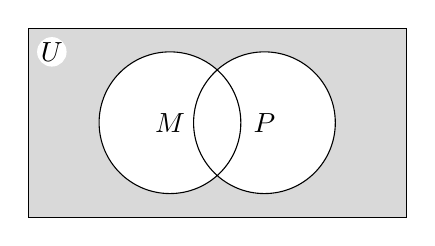
\begin{tikzpicture}[scale = 0.6]
        \filldraw [gray!30] (-3,-2) rectangle (5,2);
        \filldraw [white] (-2.5,1.5) circle (0.3);
        \draw (-2.5,1.5) node {$U$};
        \filldraw [white] (0,0) circle (1.5);
        \filldraw [white] (2,0) circle (1.5);
        \draw (0,0) circle (1.5) node {$M$} (2,0) circle (1.5) node {$P$};
        \draw (-3,-2) rectangle (5,2);
    \end{tikzpicture}
\end{center}
\item 已知全集$U=\{2,4,3-a^2\}$, 集合$P=\{2,a^2-a+2\}$, $\complement_UP=\{-1\}$, 则实数$a$的取值等于\blank{50}.
\item 已知集合$A,B$都是全集$U=\{1,2,3,4\}$的子集, 若$\complement_UA\cap B=\{1\}$, $A\cap B=\{3\}$, $\complement_UA\cap \complement_UB=\{2\}$, 则$A=$\blank{50}, $B=$\blank{50}.
\item 已知全集$U=\{2,3,a^2+2a-3\}$, $A=\{b,2\}$, $\complement_UA=\{5\}$, 求实数$a$和$b$.
\item 已知全集$U=\{-4,-3,-2,-1,0,1,2,3,4\}$, 集合$A=\{-3,a^2,a+1\}$, $B=\{a-3,2a-1,a^2+1\}$, 其中$a\in \mathbf{R}$, 若$A\cap B=\{-3\}$, 求$\complement_U(A\cup B)$.
\item 记全集$U=\{\text{三角形}\}$, $A=\{\text{锐角三角形}\}$, $B=\{\text{钝角三角形}\}$, $C=\{\text{直角三角形}\}$, $D=\{\text{斜三角形}\}$, 求$\complement_U(A\cup B)\cap \complement_U(C\cup D)$.
\item 已知全集$U=\{\text{小于}10\text{的自然数}\}$, 其子集$A,B$满足$\complement_UA\cap \complement_UB=\{1,9\}$, $A\cap B=\{2\}$, $\complement_UA\cap B=\{4,6,8\}$, 求集合$A$和$B$.
\item 下列语句哪些不是命题? 哪些是命题? 如果是命题, 那么它们是真命题还是假命题? 为什么?\\
(1) 你到过北京吗?\\
(2) 当$x=4$时, $2x<0$;\\
(3) 若$x\in \mathbf{R}$, 则方程$x^2-x+1=0$无实数根;\\
(4) $1+2=5$或$3\ge 3$;\\
(5) $x<-2$或$x>2$;\\
\item 试写出下列命题的逆命题、否命题与逆否命题, 并判断其真假:\\
命题$A$: 负数的平方是正数;\\
命题$B$: 已知$a,b$是实数, 若$a+b$是无理数, 则$a,b$都是无理数.
\item 写出下列命题的否定式:\\
(1) 不论$k$取何实数, $x^2+x+k=0$必有实数根;\\
(2) 三角形中至多有一个钝角;\\
(3) 正$n(n\ge 3)$边形的$n$个内角全相等;\\
(4) 张三是科大或北大的学生;\\
(5) 如果$x^2-x-2=0$, 那么$x\ne -1$且$x\ne -2$.
\item 判断下列命题的真假:
(1) 命题``在$\triangle ABC$中, 如果$AB>AC$, 那么$\angle C>\angle B$''的逆命题;\\
(2) 命题``如果$ab=0$, 那么$b=0$''的否命题;\\
(3) 命题``如果$a\ne 0$且$b\ne 0$, 那么$ab\ne 0$''的逆否命题;\\
(4) 命题``如果$a\ne 0$或$b\ne 0$, 那么$a^2+b^2>0$''的逆否命题.
\item 下列说法是否正确? 为什么?\\
(1) $x^2=y^2\Rightarrow x=-y$;\\
(2) $x^2\ne y^2\Rightarrow x\ne y$或$x\ne -y$.
\item 已知命题$\alpha$: 方程$x^2+mx+1=0$有两个相异负实数根, 命题$\beta$: $4x^2+4(m-2)x+1=0$无实数根, 命题$\alpha,\beta$有且只有一个为真命题, 求实数$m$的取值范围.
\item 命题``如果$a,b$都是偶数, 那么$a+b$是偶数''的逆否命题是\bracket{20}.
\onech{如果$a,b$都不是偶数, 那么$a+b$不是偶数}{如果$a,b$不都是偶数, 那么$a+b$不是偶数}{如果$a+b$不是偶数, 那么$a,b$都不是偶数}{如果$a+b$不是偶数, 那么$a,b$不都是偶数}
\item 命题``如果$p$不正确, 那么q正确''的逆命题的等价命题是\bracket{20}.
\onech{如果$q$不正确, 那么$p$不正确}{如果$q$不正确, 那么$p$正确}{如果$p$正确, 那么$q$不正确}{如果$p$不正确, 那么$q$不正确}
\item 如果命题$p$的逆命题是$q$. 命题$p$的逆否命题是$r$, 那么$q$是$r$的\bracket{20}.
\fourch{逆命题}{否命题}{逆否命题}{以上判断都不正确}
\item $(x+y)(y+z)(z+x)=0$的含义是\bracket{20}.
\twoch{$x,y,z$中有两个零}{$x,y,z$两两互为相反数}{$x,y,z$中至少有一个零}{$x,y,z$中至少有两个互为相反数}
\item 对于命题$\alpha$: ``如果$a<3$, 那么$a>1$'', 则命题$\alpha$和它的逆命题、否命题、逆否命题中真命题的个数是\bracket{20}.
\fourch{$0$}{$1$}{$2$}{$3$}
\item 已知命题``非空集合$M$的元素都是集合$P$的元素''是假命题, 给出下列命题: \textcircled{1} $M$中的元素都不是$P$的元素; \textcircled{2} $M$中有不属于$P$的元素; \textcircled{3} $M$中有$P$的元素; \textcircled{4} $M$中的元素不都是$P$的元素. 其中假命题的个数是\bracket{20}.
\fourch{$1$}{$2$}{$3$}{$4$}
\item 给出下列命题: \textcircled{1} ``如果$x+y=0$, 那么$x,y$互为相反数''的逆命题; \textcircled{2} ``全等三角形的面积相等''的否命题; \textcircled{3} ``如果$q\le 1$, 那么$x^2+2x+q=0$有实数根''的逆否命题; \textcircled{4} ``不等边三角形的三个内角相等''的逆命题. 其中真命题的序号为\bracket{20}.
\fourch{\textcircled{1}\textcircled{2}}{\textcircled{2}\textcircled{3}}{\textcircled{1}\textcircled{3}}{\textcircled{3}\textcircled{4}}
\item 命题``末位数是0的整数, 可以被5整除''的逆命题是\blank{50}.
\item 命题``线段的垂直平分线上的点与这条线段两个端点的距离相等''的否命题是\blank{50}.
\item 命题``到圆心的距离不等于圆的半径的直线不是圆的切线''的逆否命题是\blank{50}.
\item 若一个命题的否命题为``如果$x+y\le 0$, 那么$x\le 0$或$y\le 0$'', 则相应的原命题是\blank{50}.
\item 若$p:\dfrac 1{x^2-1}>0$, 则$\overline p$为\blank{50}.
\item 已知命题$p:$存在$x\in \mathbf{R}$, 使得$x^2+2ax+a\le 0$, 若命题$p$是假命题, 则实数$a$的取值范围是\blank{50}.
\item 已知命题$A:$如果$m>0$, 那么关于$x$的方程$x^2+x-m=0$有实数根.
试写出命题$A$的逆命题、否命题和逆否命题, 并判断其真假.
\item 判断命题``如果$xy\le 8$, 那么$x\le 2$且$y\le 4$''的逆命题的真假.
\item 已知命题$A:$如果$a^2+2ab+b^2+a+b-2\ne 0$, 那么$a+b\ne 1$, 求证: 命题$A$是真命题.
\item 已知$\alpha :|a-1|<2$, $\beta:$方程$x^2+(a+2)x+1=0(x\in \mathbf{R})$没有正根, 求实数$a$的取值范围, 使$\alpha,\beta$有且只有一个为真命题.
\item 已知关于$x$的方程$(x^2-1)^2-|x^2-1|+k=0$. 判断下列命题的真假:\\
(1) 存在实数$k$, 使得方程恰有$2$个不同的实数根;\\
(2) 存在实数$k$, 使得方程恰有$4$个不同的实数根;\\
(3) 存在实数$k$, 使得方程恰有$5$个不同的实数根;\\
(4) 存在实数$k$, 使得方程恰有$8$个不同的实数根.
\item 如果$a,b,c$都是实数, 那么``$ac<0$''是``关于$x$的方程$ax^2+bx+c=0$有一个正根和一个负根''的\bracket{20}.
\twoch{必要不充分条件}{充分不必要条件}{充要条件}{既不充分也不必要条件}
\item 已知$p:1\le x\le 4$, $q:\dfrac 1{x^2-x-12}>0$, 试问: $p$是$\overline q$的什么条件? 请说明理由.
\item 设$\alpha ,\beta$是方程$x^2-ax+b=0$的两个实数根, 试分析``$a>2$且$b>1$''是``两根$\alpha ,\beta$均大于$1$''的什么条件.
\item 已知$p:|x-3|\le 2$, $q:(x-m+1)(x-m-1)\le 0$, 若$\overline p$是$\overline q$的充分不必要条件, 求实数$m$的取值范围.
\item 已知集合$A=\{x|x<-3\text{或}x>5\}$, $B=\{x|a\le x\le 8\}$.\\
(1) 求实数$a$的取值范围, 使它成为$A\cap B=\{x|5<x\le 8\}$的充要条件;\\
(2) 求实数$a$的一个值, 使它成为$A\cap B=\{x|5<x\le 8\}$的一个充分不必要条件;\\
(3) 求实数$a$的一个值, 使它成为$A\cap B=\{x|5<x\le 8\}$的一个必要不充分条件.
\item 已知$a:0\le x<3$, $\beta:-1<x\le 4$, $\gamma:2x^2+mx-1<0$.\\
(1) 若$a$是$\gamma$的充分条件, 求实数$m$的取值范围;\\
(2) 若$\beta$是$\gamma$的充分条件, 求实数$m$的取值范围.
\item 已知$\triangle ABC$的三边为$a,b,c$求证: 关于$x$的方程$x^2+2ax+b^2=0$与$x^2+2cx-b^2=0$有公共根的充要条件是$A=90^\circ$.
\item ``$m=2$''是``函数$f(x)=x^2+mx-3$有两个零点''的\bracket{20}.
\twoch{充分不必要条件}{必要不充分条件}{充要条件}{既不充分也不必要条件}
\item ``$a\ne 1$或$b\ne 2$''是``$a+b\ne 3$''的\bracket{20}.
\twoch{充分不必要条件}{必要不充分条件}{充要条件}{既不充分也不必要条件}
\item 如果$x,y\in \mathbf{R}$, 那么``$x>1$或$y>2$''是``$x+y>3$''的\bracket{20}.
\twoch{充分不必要条件}{必要不充分条件}{充要条件}{既不充分也不必要条件}
\item ``$\dfrac{x^2+x+1}{3x+2}<0$''是``$3x+2<0$''的\bracket{20}.
\twoch{充分不必要条件}{必要不充分条件}{充要条件}{既不充分也不必要条件}
\item $a,b,c$三个数不全为零的充要条件是\bracket{20}.
\twoch{$a,b,c$三个数都不是零}{$a,b,c$三个数中之多有一个是零}{$a,b,c$三个数中只有一个是零}{$a,b,c$三个数中至少有一个不是零}
\item 已知$p:x^2+x-2>0$, $q:x>a$.若q是p的充分不必要条件, 则实数$a$的取值范围是\bracket{20}
\fourch{$a\ge 1$}{$a\ge 1$}{$a\ge -1$}{$a\le -3$}
\item 方程$ax^2+2x+1=0$至少有一个负实数根的充要条件是\bracket{20}.
\fourch{$0<a\le 1$}{$a>1$}{$a\le 1$}{$0<a\le 1$或$a<0$}
\item 若集合$A=\{-1,1\}$, $B=\{x|mx=1\}$, 且$B\subseteq A$, 则实数$m$的值为\bracket{20}.
\fourch{$1$}{$-1$}{$1$或$-1$}{$1$或$-1$或$0$}
\item 给出下列命题: \textcircled{1} ``$x+y=0$''是``$x^2-y^2+x+y=0$''的充分不必要条件; \textcircled{2} ``$a-b<0$''是``$a^2-b^2<0$''的充分不必要条件; \textcircled{3} ``$a-b<0$''是``$a^2-b^2<0$''的必要不充分条件; \textcircled{4} ``两个三角形全等''是``两边和夹角对应相等''的充要条件.
其中属真命题的是\bracket{20}.
\fourch{\textcircled{1}\textcircled{2}}{\textcircled{1}\textcircled{3}}{\textcircled{2}\textcircled{3}}{\textcircled{1}\textcircled{4}}
\item 有限集合$S$中元素的个数记作$\mathrm{card}(S)$, 设$A$, $B$都是有限集合, 给出下列命题:
\textcircled{1} $A\cap B=\varnothing$的充要条件是$\mathrm{card}(A\cup B)=\mathrm{card}(A)+\mathrm{card}(B)$; \textcircled{2} $A\subseteq B$的必要不充分条件是$\mathrm{card}(A)\le \mathrm{card}(B)$; \textcircled{3} $A\subseteq B$的充分不必要条件是$\mathrm{card}(A)\le \mathrm{card}(B)$; \textcircled{4} $A=B$的充要条件是$\mathrm{card}(A)=\mathrm{card}(B)$. 
其中真命题的个数是\bracket{20}.
\fourch{$0$}{$1$}{$2$}{$3$}
\item 已知集合$A=\{-1,3,2m-1\}$, $B=\{3,m^2\}$, 若$B\subseteq A$, 则实数$m=$\blank{50}.
\item 已知$p$是$r$的充分不必要条件, $s$是$r$的必要条件, $q$是$s$的必要条件, 那么$p$是$q$的\blank{50}条件.
\item 指出下列各命题中, $p$是$q$的什么条件:\\
(1) $p:0<x<3$, $q:|x-1|<2$;\\
(2) $p:(x-2)(x-3)=0$, $q:x=2$;\\
(3) $p:c=0$, $p$: 抛物线$y=ax^2+bx+c$过原点;\\
(4) $p:A\subseteq B\subseteq U$, $q:\complement_UB\subseteq A$.
\item ``$xy>0$''的一个充分不必要条件是\blank{50}.
\item ``$\sqrt x>\sqrt y$''的一个必要不充分条件是\blank{50}.
\item ``$a^2+b^2>0$''的\blank{50}条件是``$a\ne 0$''.
\item 若$p:x\ne 2$且$y\ne 3$, $q:x+y\ne 5$, 则是$p$是$q$成立的\blank{50}条件.
\item 若集合$A=\{x|x^2+x-6=0\}$, $B=\{x|mx+1=0\}$, 则$B$是$A$的真子集的一个充分不必要条件是\blank{50}.
\item 已知$p:\sqrt{x-1}>0$, $q:|x|=-x$, 试问: $p$是$\overline q$的什么条件? 请说明理由.
\item 已知$m>0$, $p:-2\le x\le 10$, $q:1-m\le x\le -1+m$, 若$\overline p$是$\overline q$的必要不充分条件, 求实数$m$的取值范围.
\item 求证: ``$x+y=5$''是``$x^2+y^2-3x+7y=10$''的充分不必要条件.
\item 设$x,y\in \mathbf{R}$, 求证: $|x+y|=|x|+|y|$成立的充要条件是$xy\ge 0$.
\item 已知函数$f(x)=ax-bx^2$.\\
(1) 当$b>0$时, 若对任何$x\in \mathbf{R}$都有$f(x)\le 1$, 求证: $a\le 2\sqrt b$;\\
(2) 当$b>1$时, 求证: ``对任意$x\in [0,1]$, $|f(x)|\le 1$''的充要条件是$b-1\le a\le 2\sqrt b$.
\end{enumerate}
\end{document}